\documentclass[11pt]{article}
\usepackage[utf8]{inputenc}
\usepackage[a4paper, margin=1in]{geometry}
\usepackage{graphicx}
\usepackage{amssymb}
\usepackage{gensymb} % for advanced symbols
\usepackage{amsmath}
\usepackage{amssymb}
\usepackage{multicol}
\setlength{\columnsep}{1cm}
\usepackage{wrapfig}
\usepackage{float}
\usepackage{appendix}
\usepackage{hyperref}
\usepackage{float}

\graphicspath{ {Images/} }
\hypersetup{
    colorlinks=true,
    linkcolor=blue,
    filecolor=magenta,      
    urlcolor=blue,
    pdftitle={Overleaf Example},
    pdfpagemode=FullScreen,
    }
\urlstyle{same}

\begin{document}

\begin{center}
\textbf{Department of Electronic and Telecommunication Engineering\\[10 pt]University of Moratuwa \\[20 pt] EN2090  Laboratory Practice - II \\[20 pt]}

\includegraphics[width=0.4\linewidth]{uom_logo.png}

\begin{huge}
\vspace{30mm}
\textbf{Project Report \\[20 pt] FUNCTION GENERATOR} \\[100 pt]
\end{huge}

\begin{tabular}{c c c }
1. & G.I. Hewasura & 190234E  \\
2. & T. Jayabawan  & 190250A  \\ 
3. & D.R. Jayasinghe & 190262L  \\  
4. & L.H.T.V. Jayawardane & 190274B
\end{tabular}

\textbf{\\[20 pt]Supervisor: Mr. Pasan Dissanayake\\[10 pt]}

\begin{large}
\today
\end{large}

\end{center}
\thispagestyle{empty} 
\newpage

\begin{multicols}{2}
[
\rule{\textwidth}{0.5pt}
\begin{abstract}
    Most of the electronics applications require various wave forms. From finding the characteristics of OPAMPs and diodes to testing the inner workings of the audio amplifier these wave forms are used. This report discusses about an analog function generator which can produce sine, square, triangular and saw tooth wave forms at the range of 20Hz to 20000Hz in frequency where the output voltage varies from -5v to 10v.
\end{abstract}
\rule{\textwidth}{0.5pt}
]
\tableofcontents

\section{Introduction}
Analog function generator is an electronic device which is implemented using the basic elements such as OPAMPs and other passive elements. This project "analog function generator" is made as a report covering the aspects of building it physically. First, the methodology used to implement the requirements is discussed. In this part the implementations with circuit diagrams and the principles are discussed. Next the results are described, for each wave forms the output through the oscilloscope are presented and the 


\section{Method}

\subsection{Waveform Generation}

\subsubsection{Square Wave with PWM}
An astable mutivibrator circuit is used in the generation process of the square wave where a Schmitt trigger logic gate is combined with a capacitor. The Schmitt trigger action changes the state between an upper and a lower threshold level as the input voltage signal increase and decrease about the input terminal. When the charge across the capacitor is higher than the Schmitt trigger higher threshold level since the voltage of the positive terminal is higher than the negative terminal, the output result to be logic “0” and vice versa. The period of the square wave changes with the R*C value, a potentiometer is used in the place of R to change the frequency. \\ The PWM signal is generated by sending the triangular waveform generated between the capacitor and the potentiometer through a comparator circuit. The duty cycle of the PWM signal is changed by varying the reference voltage in the positive terminal using the potentiometer in the comparator circuit. The PWM signal generated by the comparator  is sent through a rectifier circuit to achieve a half rectified the PWM signal.
\begin{figure}[H]
    \centering
    \includegraphics[width=0.35\textwidth]{astable_multi.png}
    \caption{Astable Multivibrator Circuit}
    \label{fig:mesh1}
\end{figure}
\begin{figure}[H]
    \centering
    \includegraphics[width=0.5\textwidth]{pwm.png}
    \caption{PWM signal genaration}
    \label{fig:mesh1}
\end{figure}
\subsubsection{Triangle Wave}
Triangular wave is extracted in between the capacitor and the potentiometer where the triangular wave is generated as a result of the charging and discharging of the capacitor.
\begin{figure}[H]
    \centering
    \includegraphics[width=0.5\textwidth]{graph.png}
    \caption{Square and triangular pulse generation}
    \label{fig:mesh1}
\end{figure}

\subsubsection{Sine Wave}
Tilan
\subsubsection{Sawtooth Wave}

In order to produce the sawtooth waveform, the magnitude should instantly come to zero from the peak value. To implement this a capacitor can be short circuited but using this the capacitor won’t charge initially. By using a transistor we can find an optimal solution. \\
Here the transistor is in cut-off region to be charged. When capacitor is charged up to required saturation level, a momentary positive pulse is applied at the base of the transistor to send it into saturation. In saturation $V_{CE} = 0$, so capacitor is short circuited and discharges quickly to zero. The positive pulses are given as a PWM signal with a very small duty cycle.

\begin{figure}[H]
    \centering
    \includegraphics[width=0.5\textwidth]{sawtooth_generator.png}
    \caption{Square and triangular pulse generation}
    \label{fig:mesh1}
\end{figure}

\subsection{Output Stage}
According to the given specifications the function generator must be able to drive 50\(\Omega\) load. In general an OPAMP can provide only upto 100mA current which is not enough to drive a 50\(\Omega\) load at 10V pk-pk. In order to accomplish this task we used an OPAMP buffer circuit containing transistor push-pull stage. The maximum current required is about 200mA (10V/50\(\Omega\)). For this we are using 2N2222A NPN and 2N2907A transistors which can support upto 800mA \(I_{C}\) current.

\begin{figure}[H]
    \centering
    \includegraphics[width=0.4\textwidth]{buffer_circuit.PNG}
    \caption{Buffer Circuit (using OPAMPS and push-pull stage}
    \label{fig:mesh1}
\end{figure}

\section{Results}
After testing the following results could be obtained relating to different modules in the function generator circuits.

\subsection{Component Selection}

Following are the main components used in the implementation of the analogue function generator.
\vspace{-2mm}

\begin{itemize}
    \setlength\itemsep{-2mm}
    \item TL084CN Quad-OPAMP
    \item AD826AN Dual-OPAMP
    \item 2N2222A, 2N2907A, 2N3904 transistors
    \item resistors, potentiometers, capacitors, etc.
\end{itemize}

\subsubsection*{TL084CN}
TL084CN is a 14-pin Quad Operational Amplifier by Texas Instruments. It has a slew rate of \(20 \; V/\mu s\) and a unity gain bandwidth of 5.25MHz. All the signal generation tasks were carried out using 2 of these OPAMPs. This OPAMPs able to produce both low (40Hz) and high (20kHz) frequency signals with sufficient accuracy.  

\subsubsection*{AD826AN}
AD826AN is an 8-pin Dual Operational Amplifier by Analog Devices. Is has a very high slew rate of \(350 V\mu s\) and a unity gain bandwidth of 40-50MHz. This OPAMP was used in the output stage as a non-inverting amplifier and a buffer before the transistor push-pull stage.


\subsection{Square and PWM wave}
We used two capacitors (\(10nF\) and \(0.33\mu F\)) to achieve lower and higher frequencies respectively in the relaxation oscillator. The PWM control is done using the OPAMP comparator. The following images show rectified square waveforms with different PWM values.

\begin{figure}[H]
    \centering
    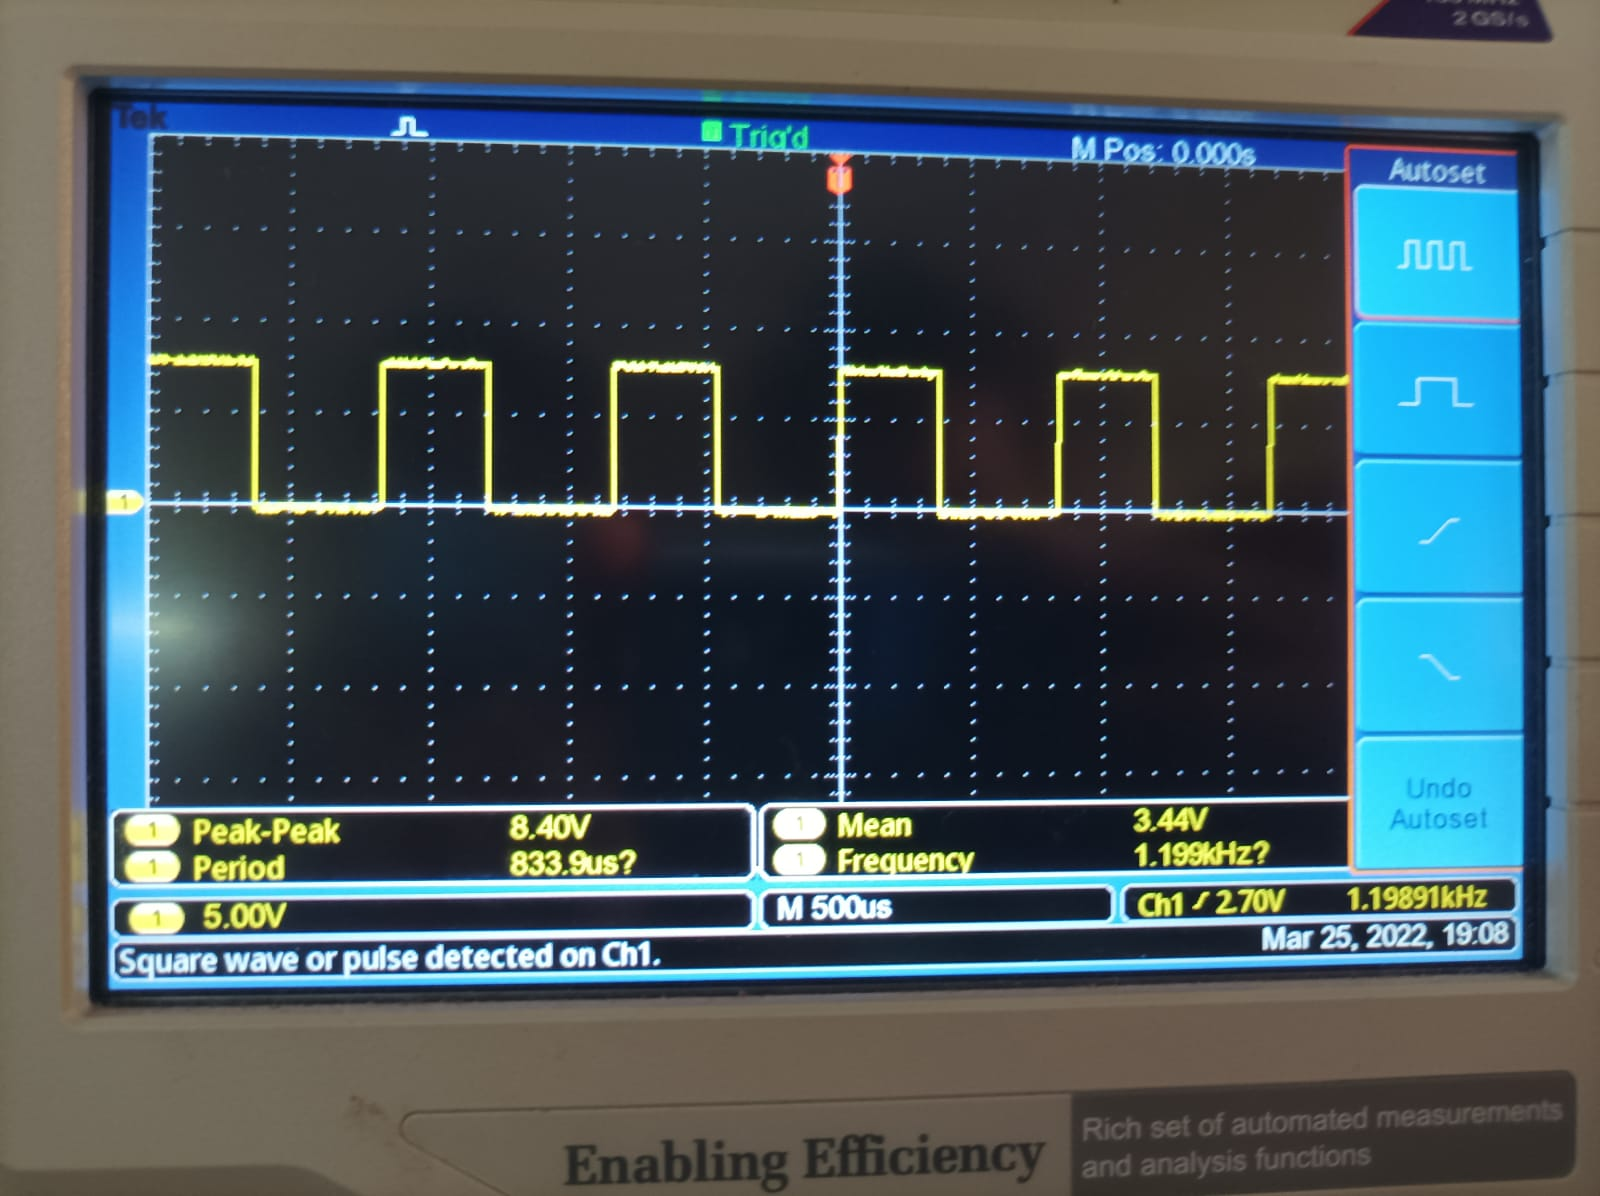
\includegraphics[width=0.4\textwidth]{Square_Wave_1kHz.jpeg}
    \caption{1kHz Square Wave Signal}
    \label{fig:mesh2}
\end{figure}

\begin{figure}[H]
    \centering
    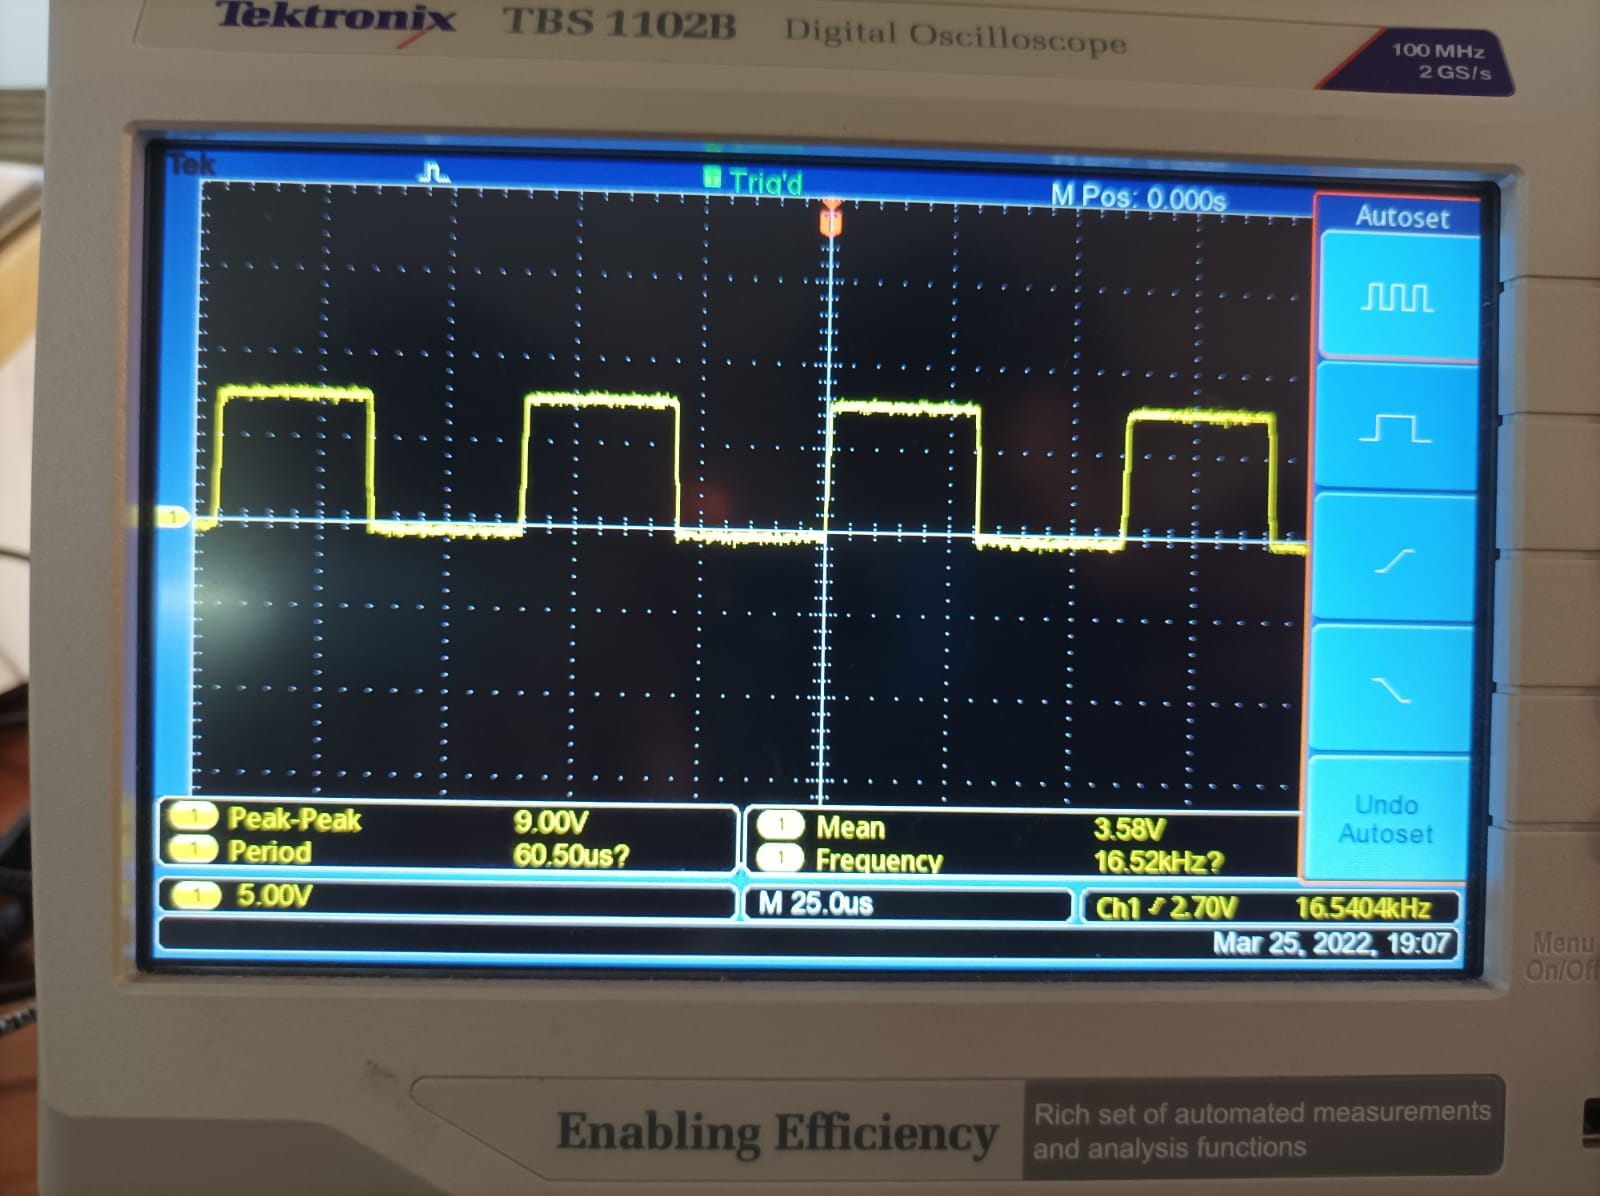
\includegraphics[width=0.4\textwidth]{Square_Wave_16kHz.jpeg}
    \caption{16kHz Square Wave Signal}
    \label{fig:mesh2}
\end{figure}

\begin{figure}[H]
    \centering
    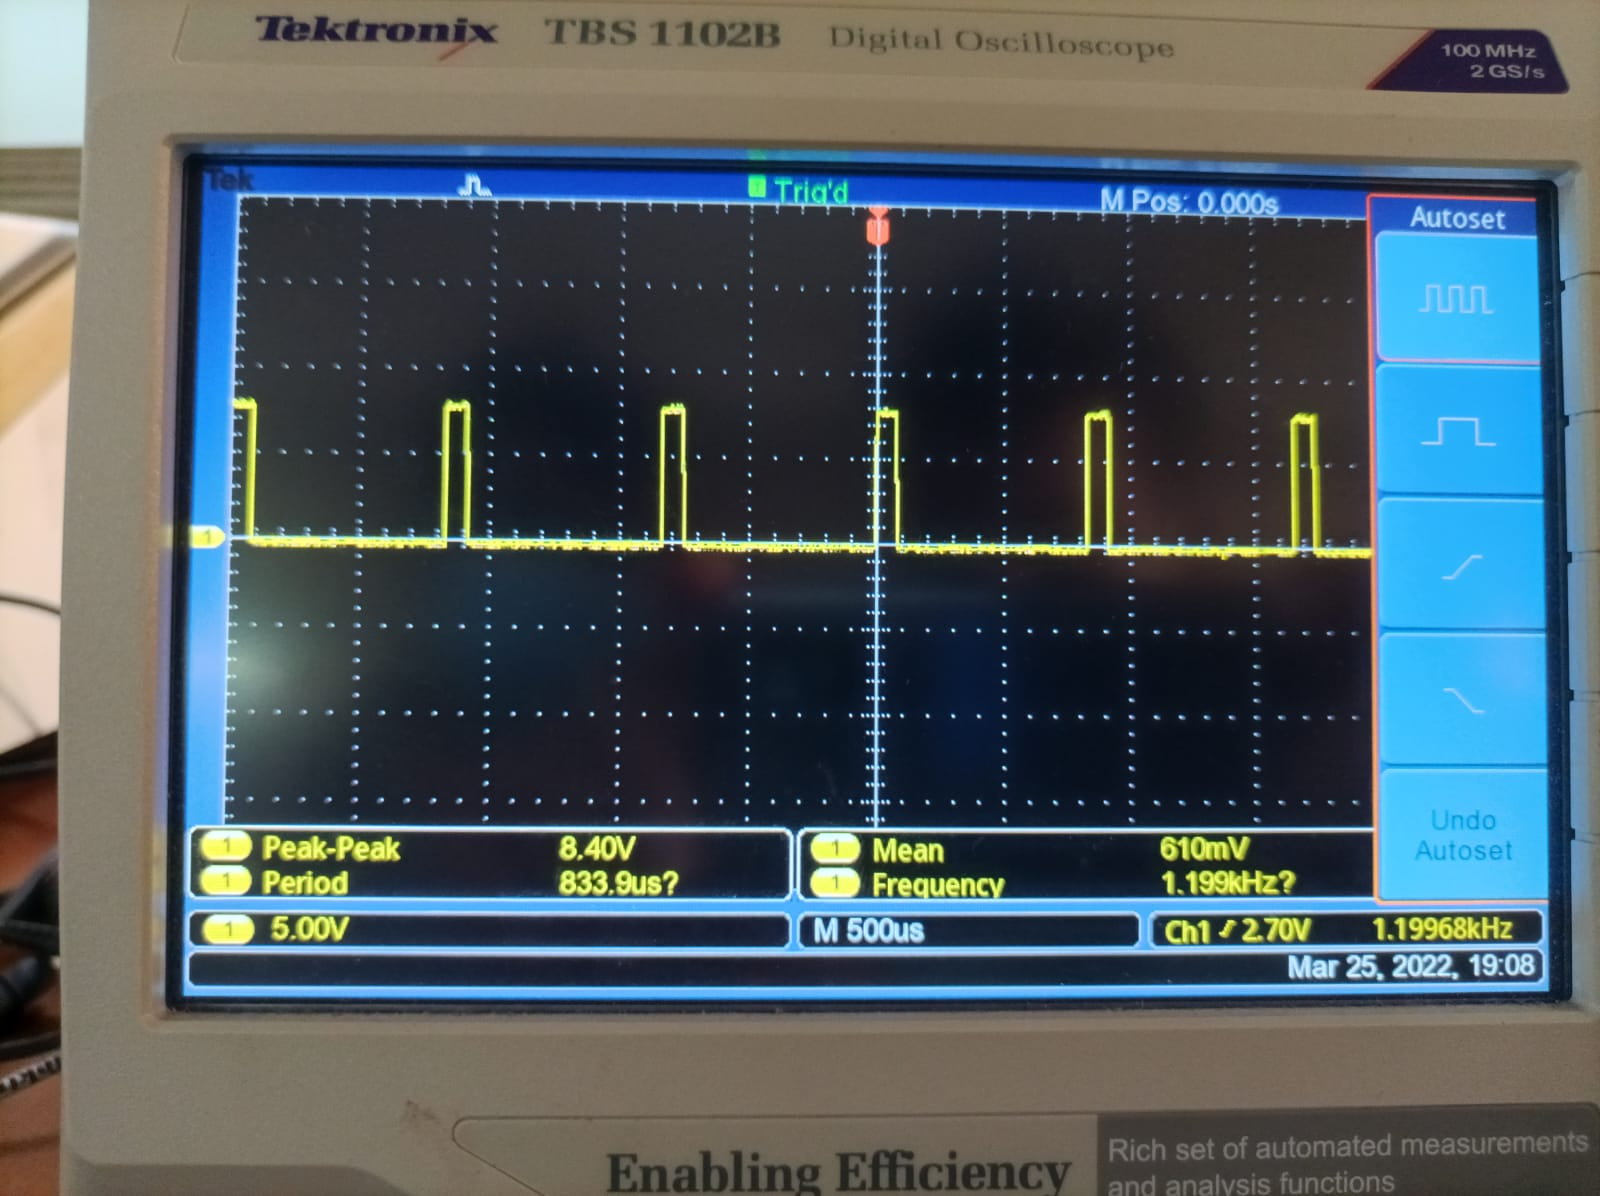
\includegraphics[width=0.4\textwidth]{PWM_1kHz.jpeg}
    \caption{PWM control of square wave}
    \label{fig:mesh3}
\end{figure}

\begin{figure}[H]
    \centering
    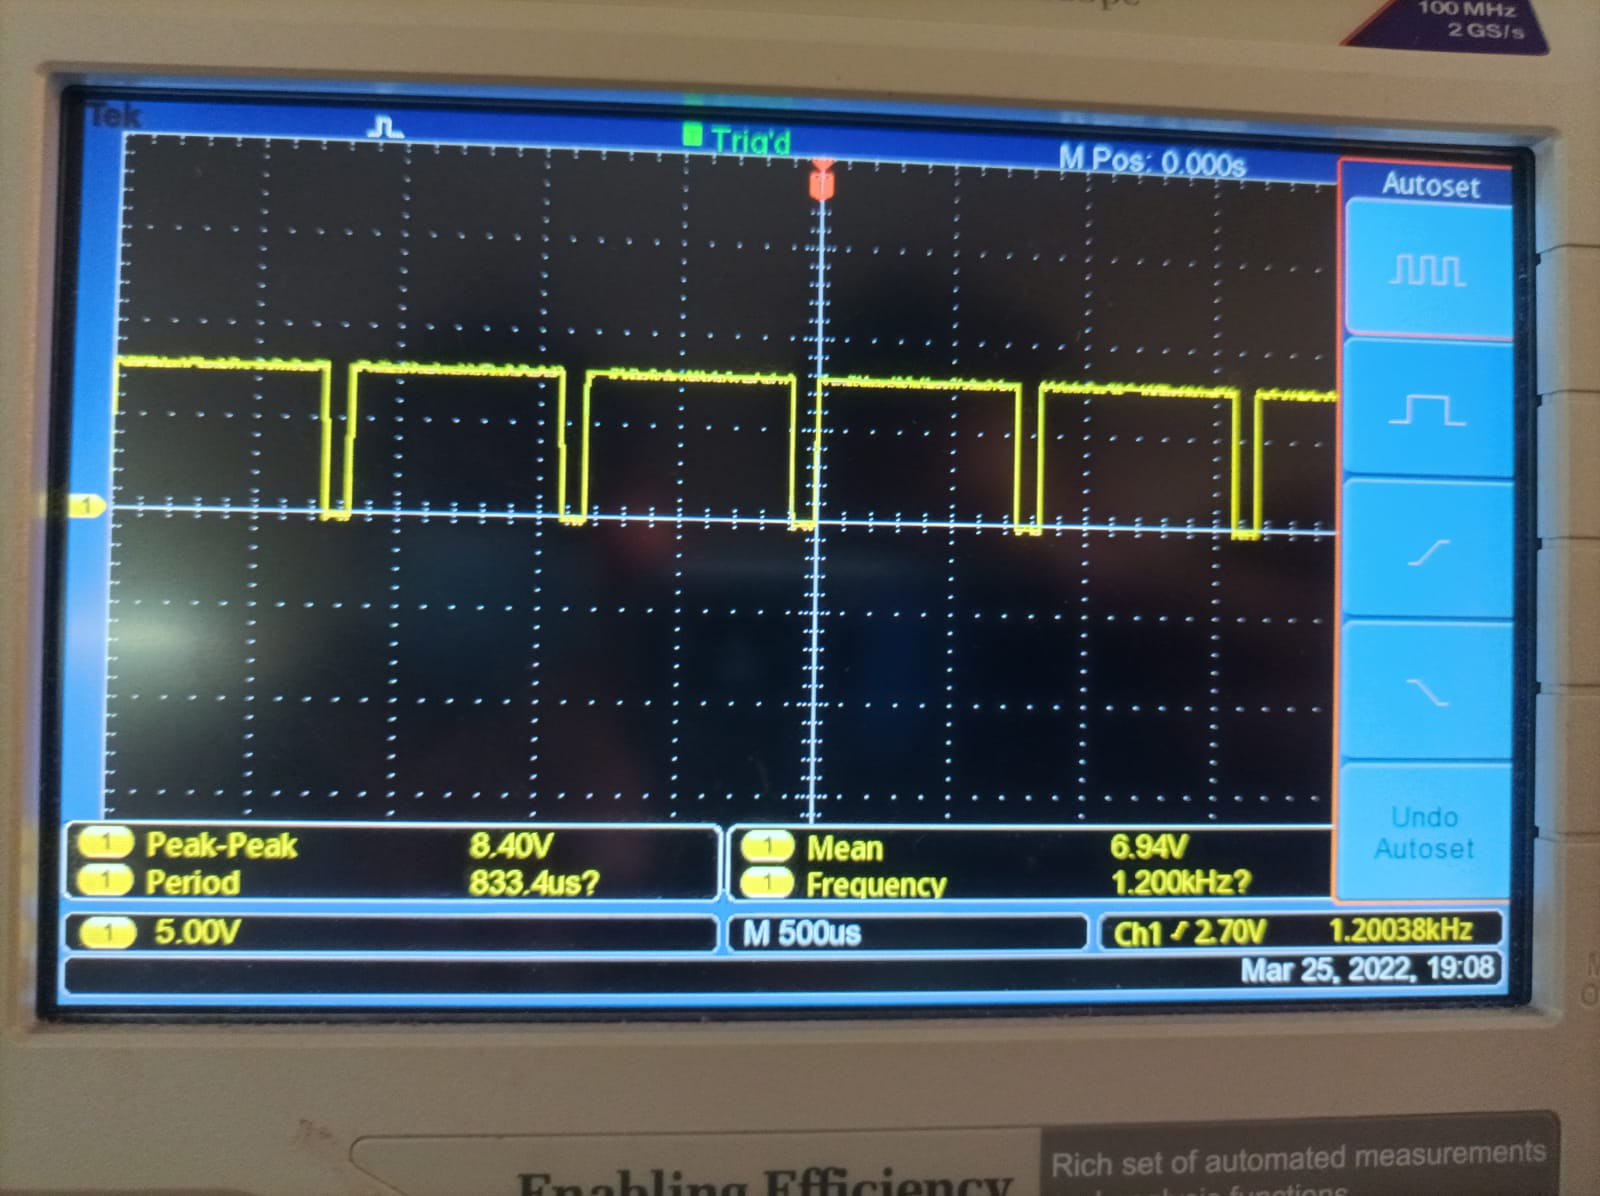
\includegraphics[width=0.4\textwidth]{PWM_1kHz_1.jpeg}
    \caption{PWM control of square wave}
    \label{fig:mesh4}
\end{figure}

\subsection*{Triangle Wave}

The triangle waveform is obtained as the voltage across the capacitor from the relaxation oscillator. 

\begin{figure}[H]
    \centering
    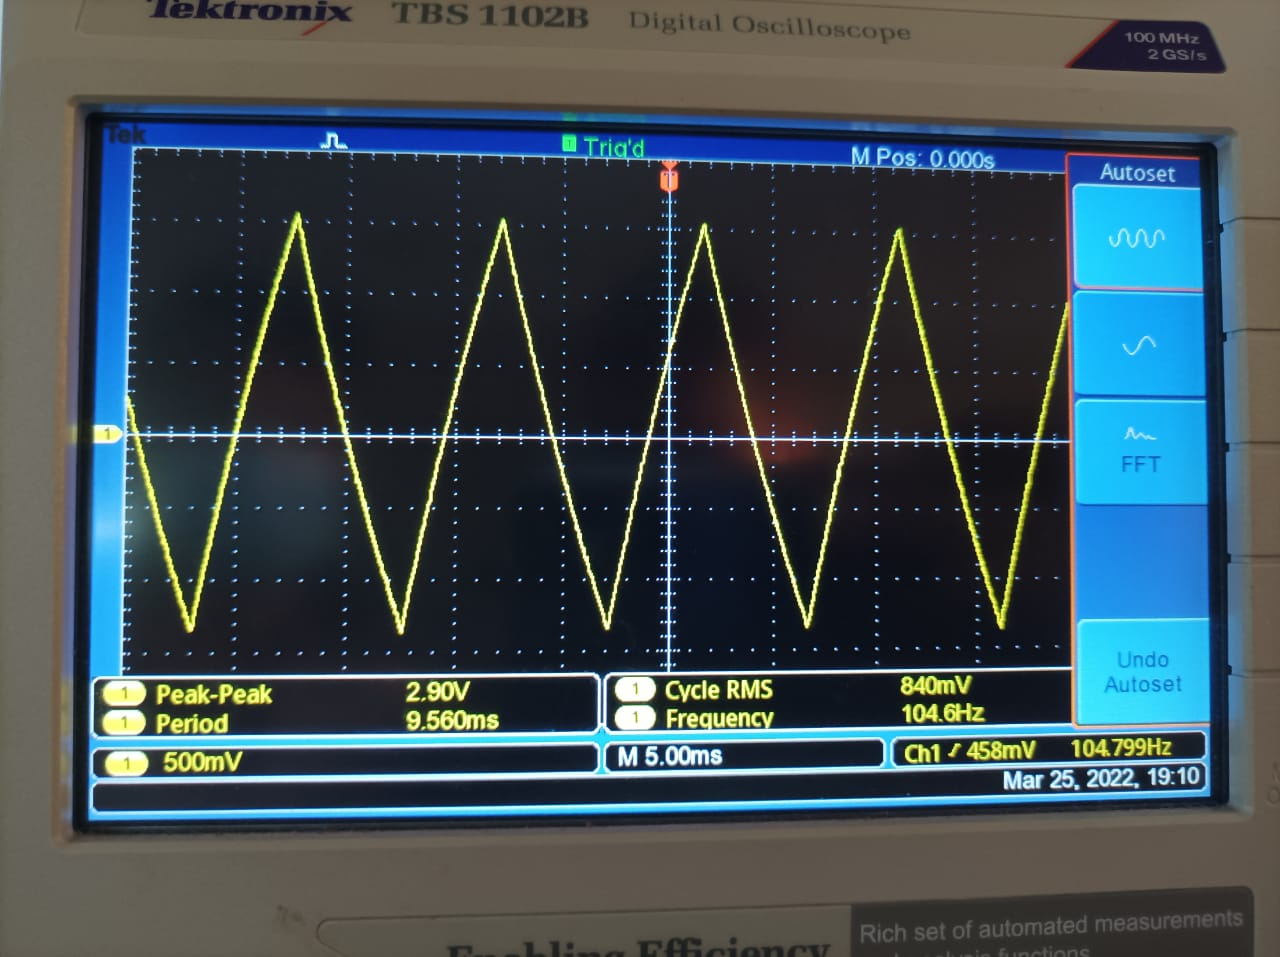
\includegraphics[width=0.4\textwidth]{Triangle_100Hz.jpeg}
    \caption{100Hz triangle waveform}
    \label{fig:mesh5}
\end{figure}

\begin{figure}[H]
    \centering
    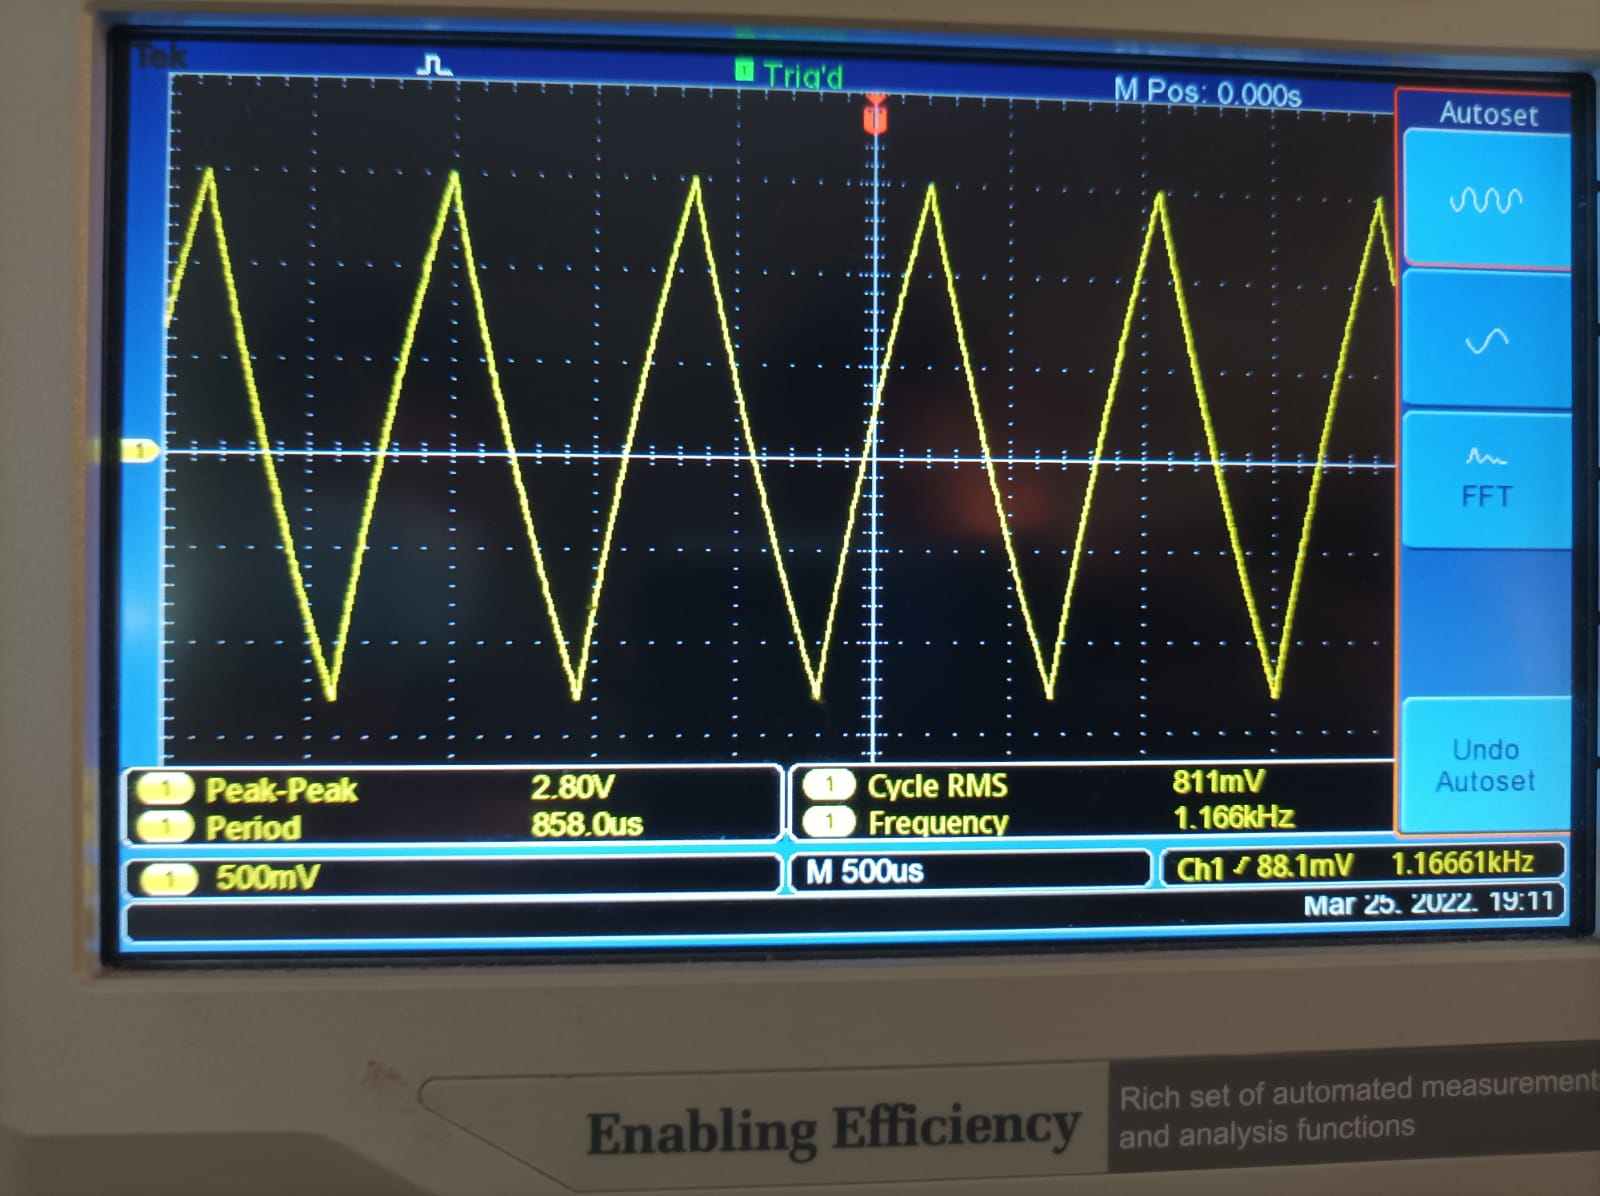
\includegraphics[width=0.4\textwidth]{Triangle_1kHz.jpeg}
    \caption{1kHz triangle waveform}
    \label{fig:mesh6}
\end{figure}

\begin{figure}[H]
    \centering
    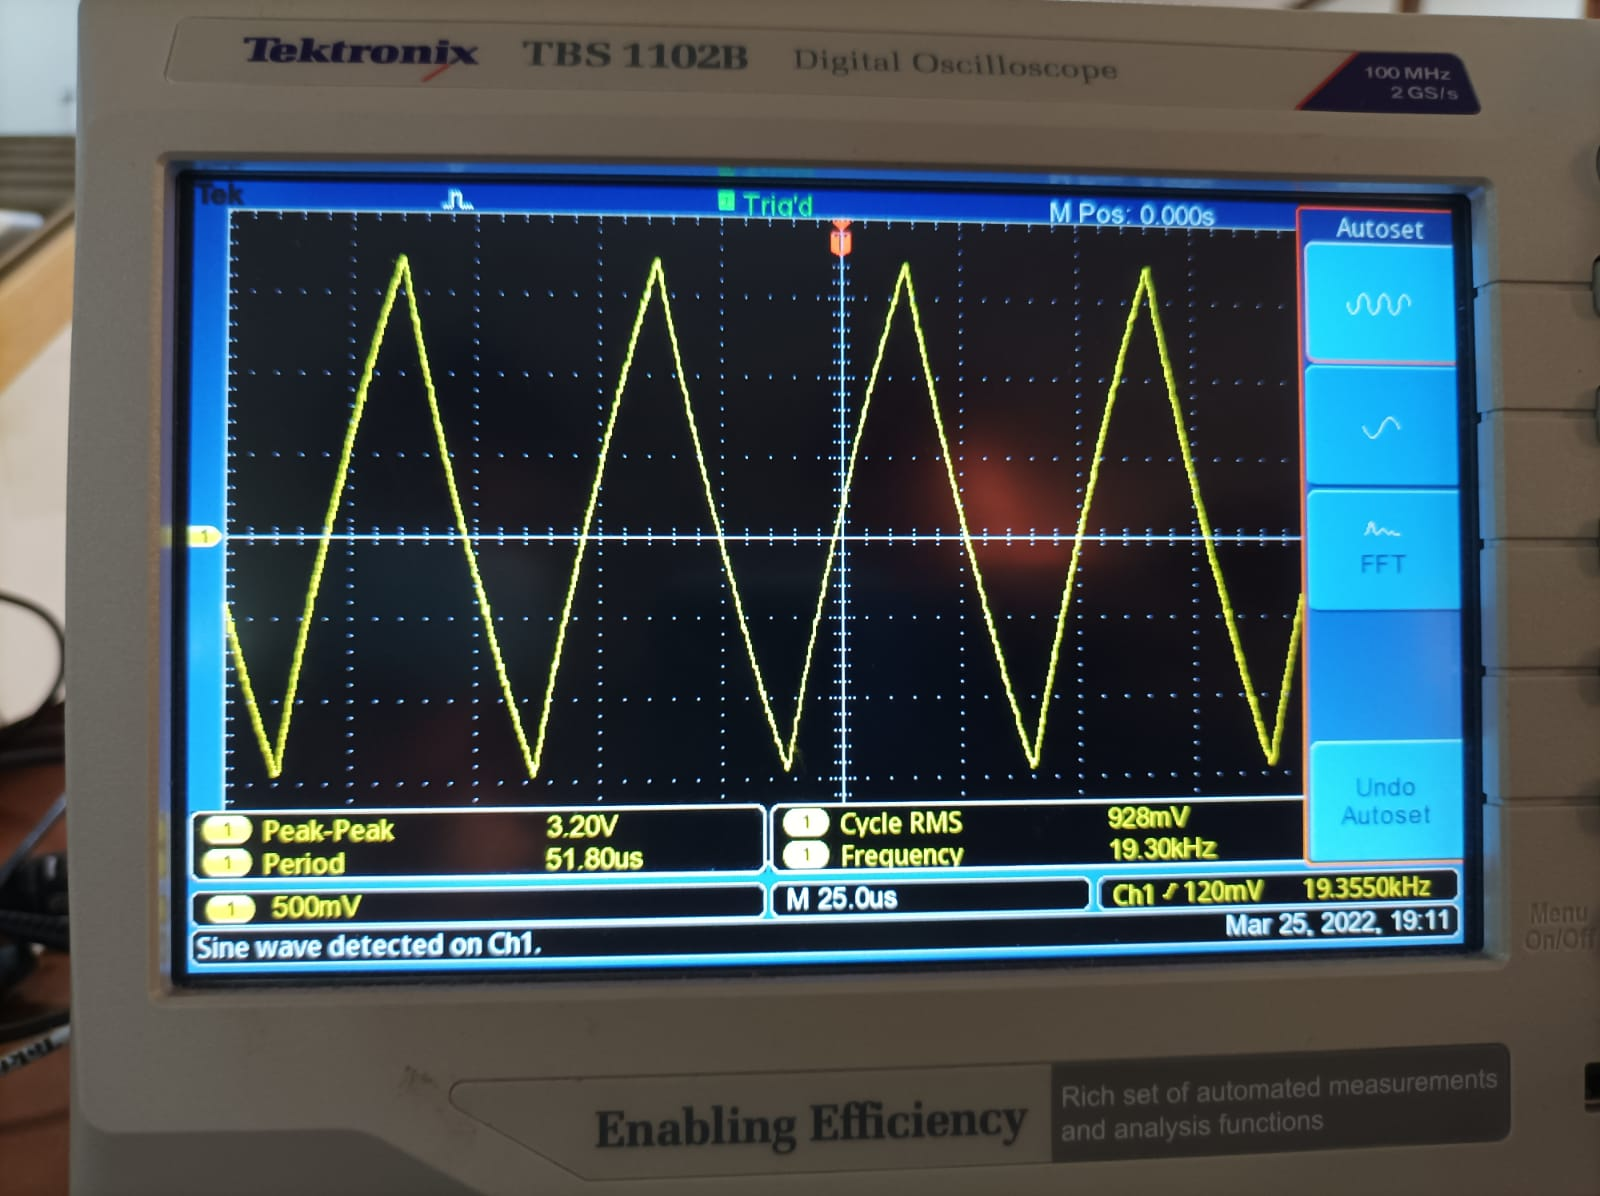
\includegraphics[width=0.4\textwidth]{Triangle_20kHz.jpeg}
    \caption{20kHz triangle waveform}
    \label{fig:mesh7}
\end{figure}

\subsection*{Sine Wave}

The sine wave is obtained after the triangle waveform is filtered from the low pass filters. From the four filters we used the accurate wave forms could be obtained.

\begin{figure}[H]
    \centering
    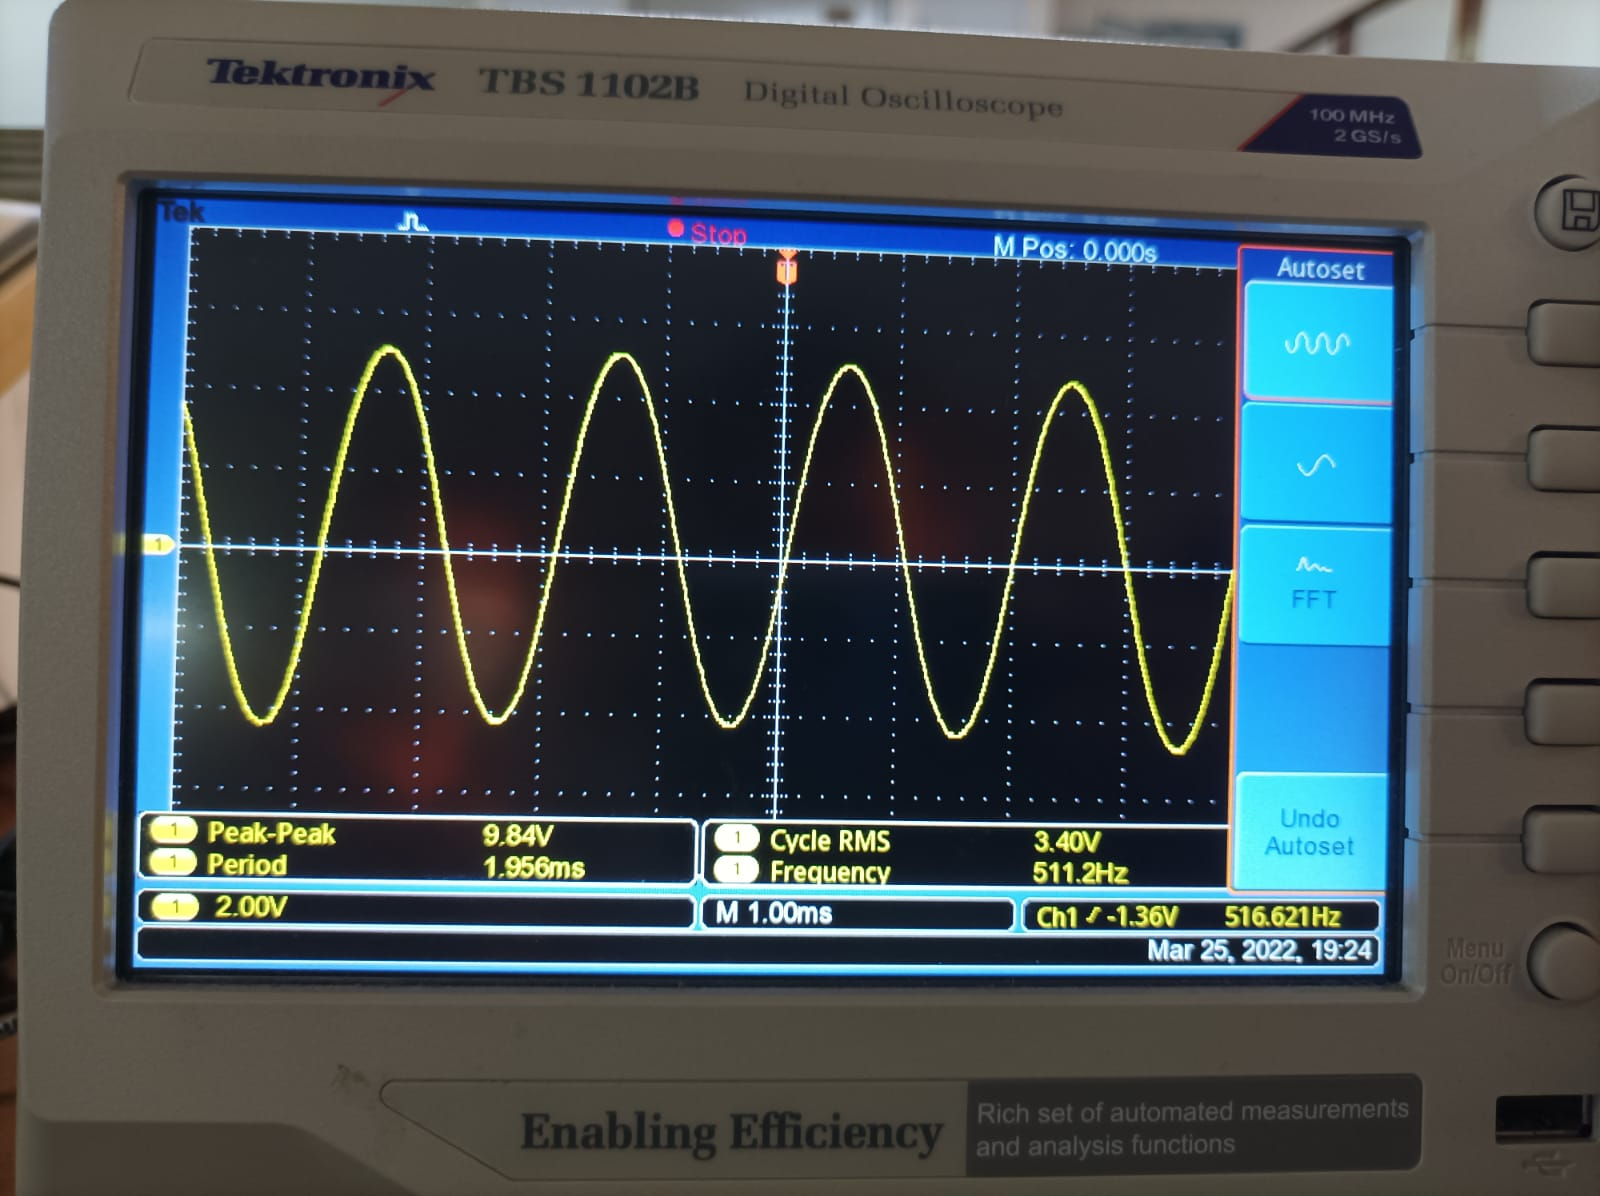
\includegraphics[width=0.4\textwidth]{Sine_500Hz.jpeg}
    \caption{500Hz sine waveform}
    \label{fig:mesh5}
\end{figure}

\begin{figure}[H]
    \centering
    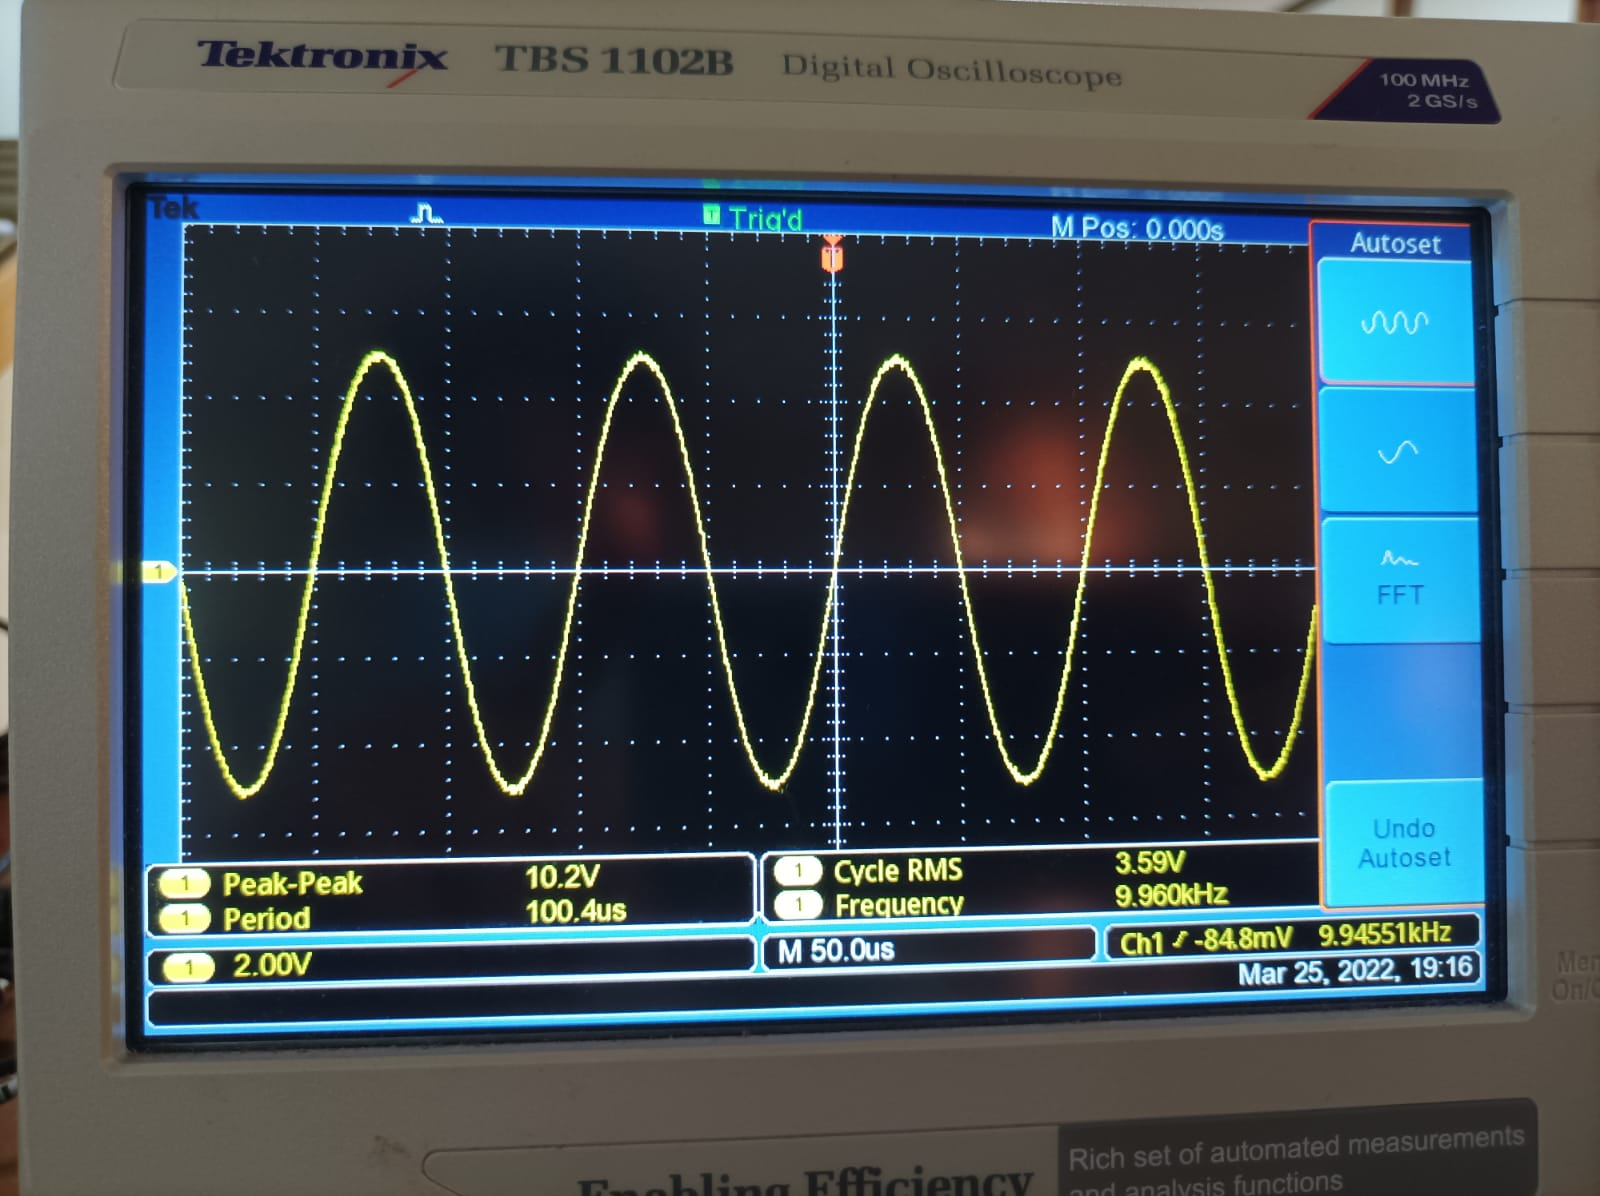
\includegraphics[width=0.4\textwidth]{Sine_10kHz.jpeg}
    \caption{10kHz sine waveform}
    \label{fig:mesh6}
\end{figure}

\begin{figure}[H]
    \centering
    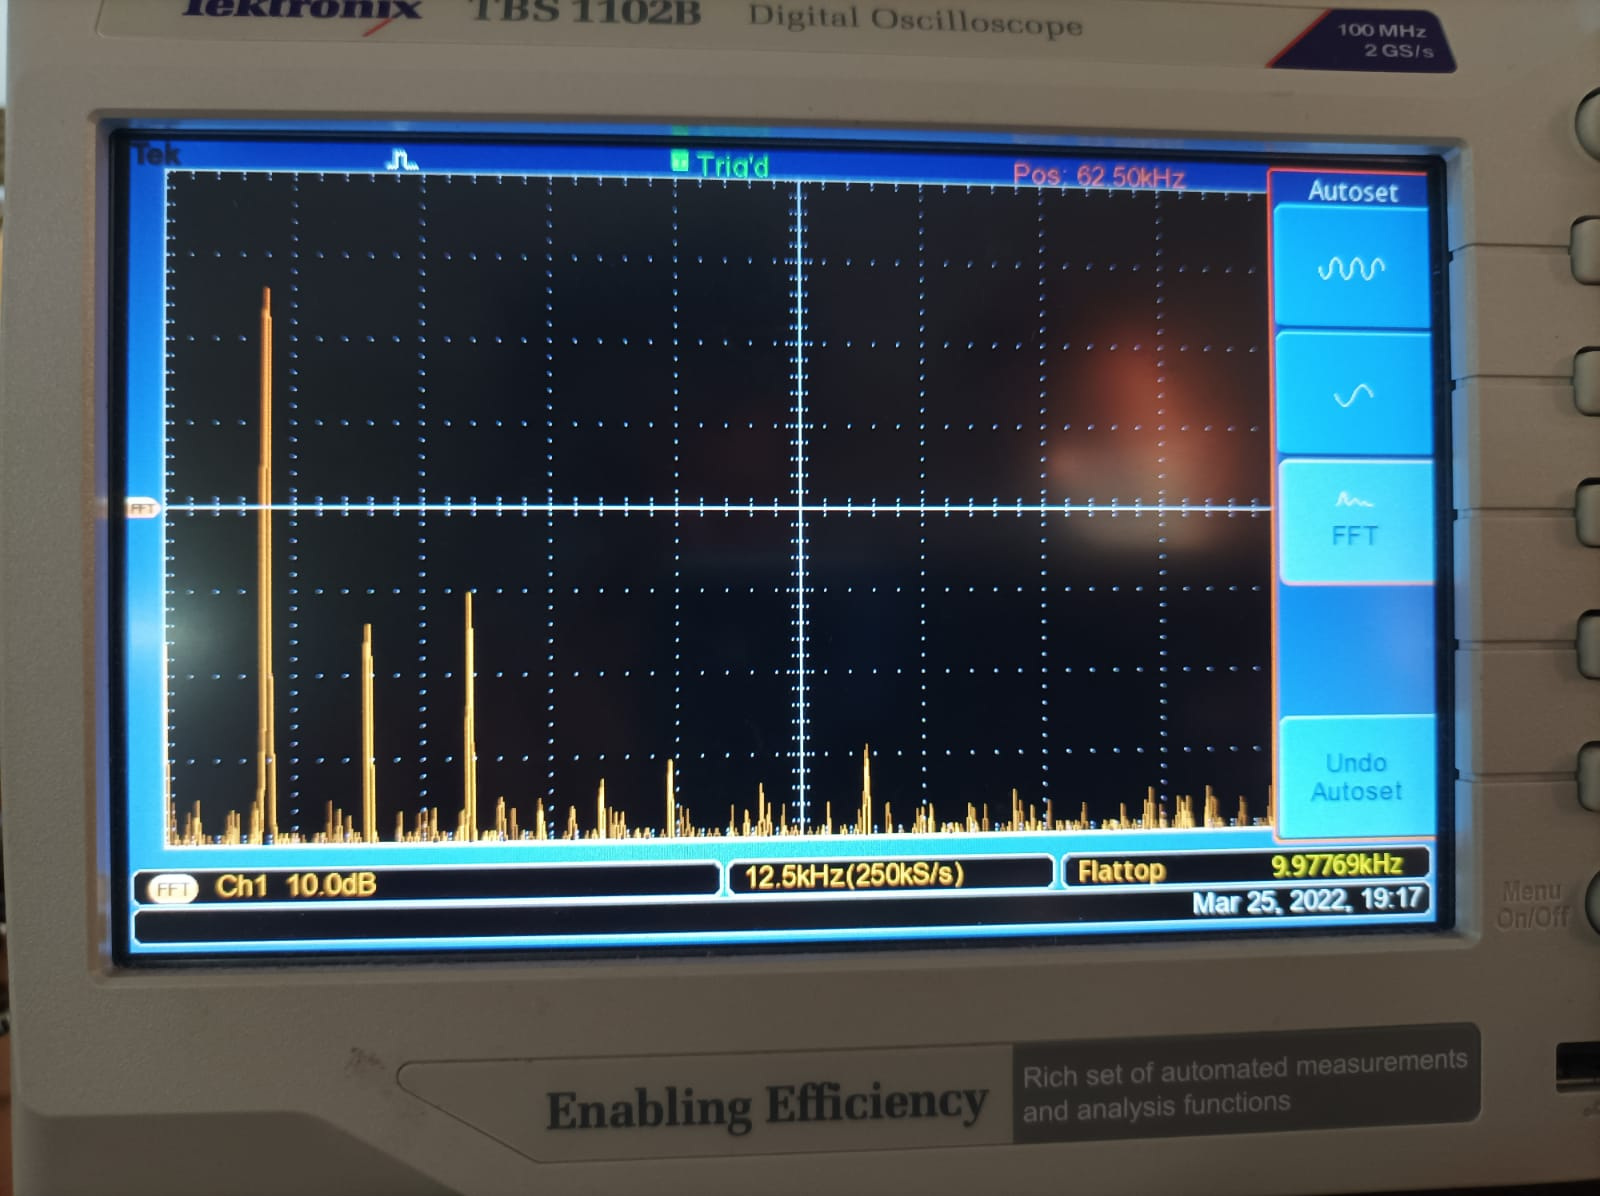
\includegraphics[width=0.4\textwidth]{Sine_FFT_10kHz.jpeg}
    \caption{Frequency spectrum of 10kHz sine waveform}
    \label{fig:mesh7}
\end{figure}

\section{Discussion}

Following are some of the issues we encountered when designing the analogue function generator. We were able to fix some these issues.

\subsubsection*{Shape of the Triangle Waveform}
The triangle wave which was obtained as the capacitor voltage of the relaxation oscillator, was not exactly triangular in shape. At closer inspection it is possible to see a curve similar to that of a capacitor charging and discharging. This could have been avoided by integrating the square wave, using an \textbf{OPAMP integrator} circuit instead. But we decided not to implement it because, the waveform was very nearly triangular. 
\\
\textbf{\textcolor{red}{image of a distorted triangle wave}}

\subsubsection*{Amplitude reduction of Sine and Sawtooth functions when increasing frequency}

This is another issue that could not be completely resolved in our design. As the frequency is increased, the amplitude of both sine and sawtooth wave reduced dramatically. This happened in each waveform due to the following reason;
\begin{itemize}
    \item \textbf{Sine wave} - Once the frequency was increased past the cutoff frequency of the filter, the gain reduction caused the amplitude of the waveform to drop. 
    \item \textbf{Sawtooth Wave} - \textbf{\textcolor{red}{Reason for the decrease in amplitude}}
\end{itemize}

The method currently used to overcome this issue is to, increase the amplitude at the output stage to counter balance the amplitude reduction resulted by frequency change.

\end{multicols}

\newpage

\section{Appendices}

\subsection{Appendix I - PCB Layout}


\begin{multicols}{2}
\begin{figure}[H]
    \centering
    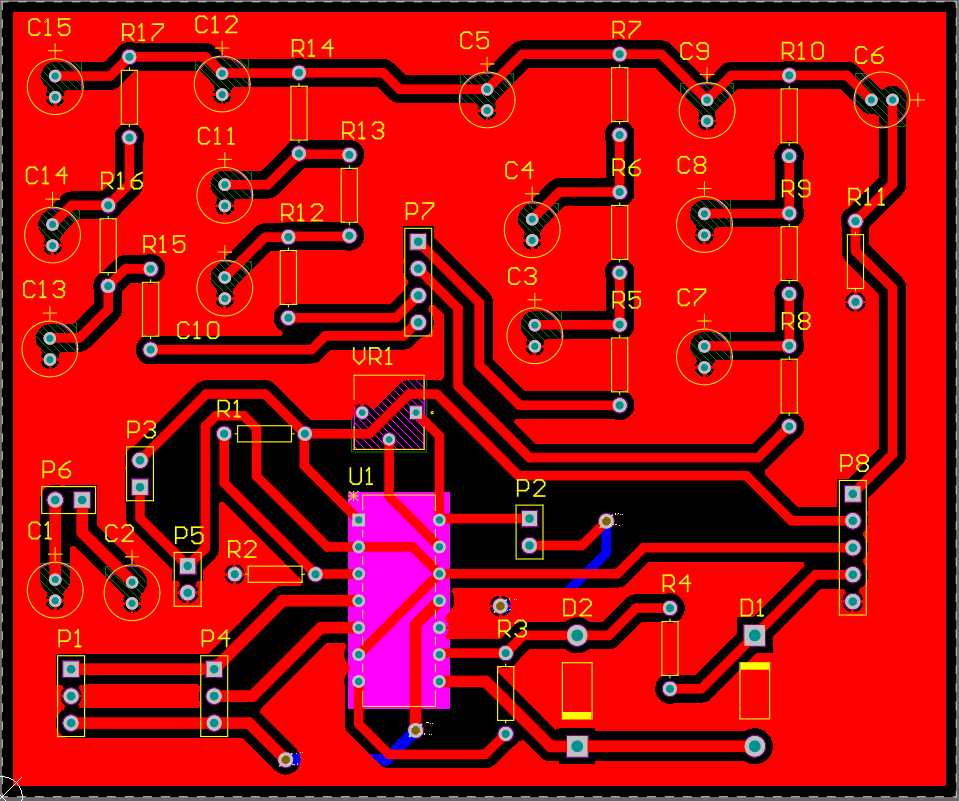
\includegraphics[width=0.5\textwidth]{pcb1_layout.PNG}
    \caption{PCB 1 - Triangle, Square, Sine Wave generation}
    \label{fig:mesh6}
\end{figure}

\begin{figure}[H]
    \centering
    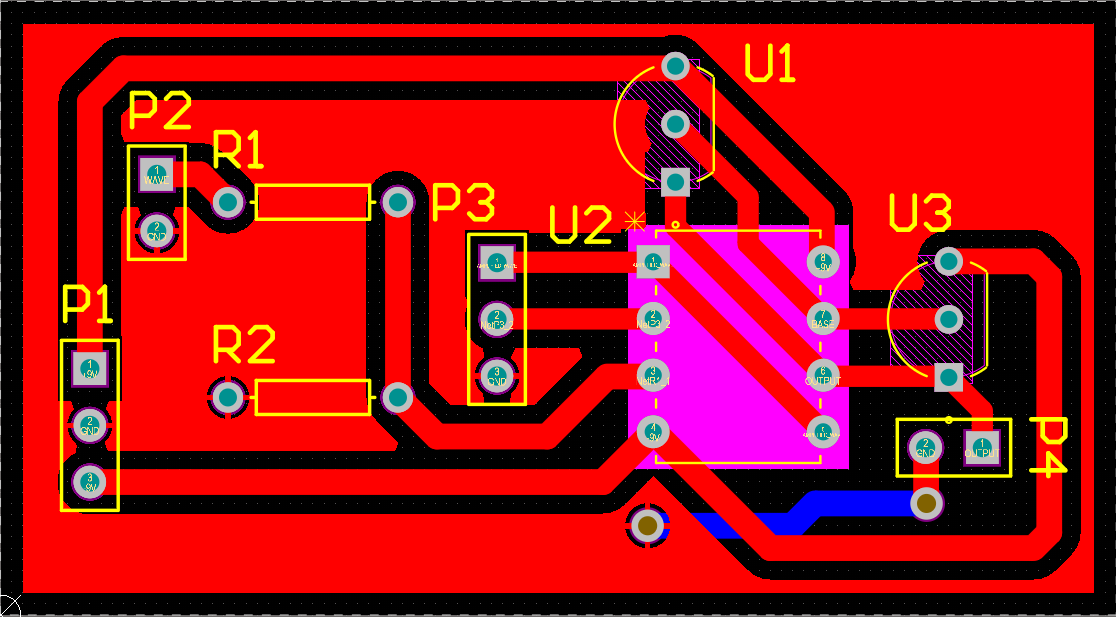
\includegraphics[width=0.5\textwidth]{pcb2_layout.PNG}
    \caption{PCB 2 - Output Stage }
    \label{fig:mesh6}
\end{figure}

\begin{figure}[H]
    \centering
    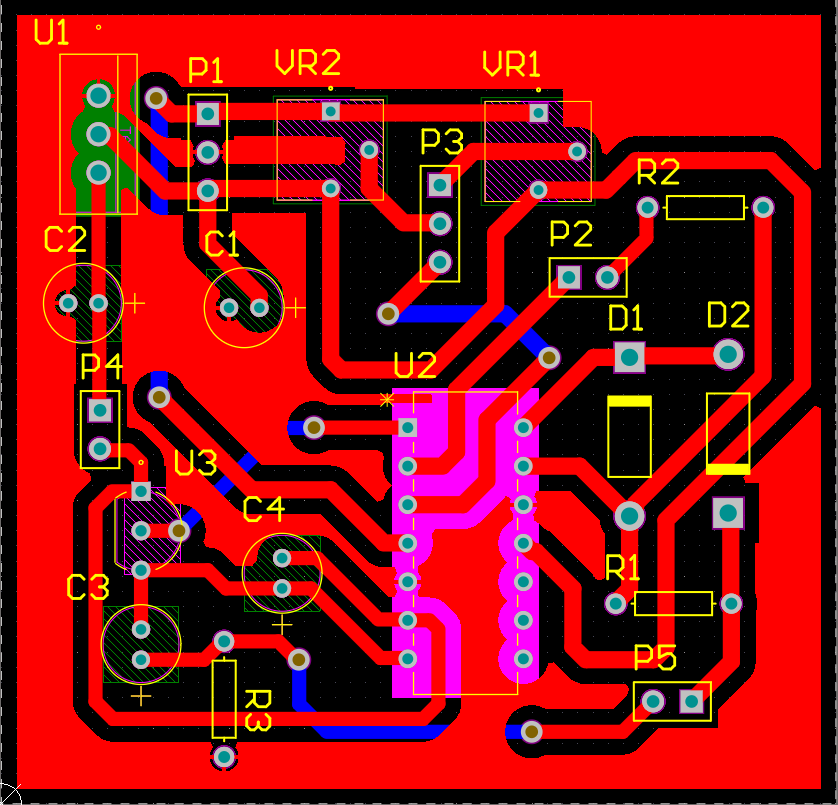
\includegraphics[width=0.5\textwidth]{pcb3_layout.PNG}
    \caption{PCB 3 - Sawtooth Wave Generation}
    \label{fig:mesh6}
\end{figure}

\end{multicols}

\section{Appendix II - Enclosure}




\newpage

\section{Appendix III - Datasheet}

\rule{\textwidth}{0.5pt}

\begin{center}
    \begin{large}
    \textbf{Analogue Function Generator - Datasheet}
    \end{large}

\end{center}

\subsection*{Features}
\begin{itemize}
    \setlength\itemsep{-2mm}
    \item 5 output functions
    \item Adjustable frequency from 40Hz to 20kHz
    \item Amplitude can be adjusted within \(\pm\)7V
    \item Can drive small loads
\end{itemize}

\subsection*{Description}

Analogue Function Generator is designed completely using analogue electronic components and it is capable of producing the following output functions.
\begin{itemize}
    \setlength\itemsep{-2mm}
    \item Triangle Wave
    \item Square Wave (50\% duty)
    \item Square Wave PWM (variable duty cycle)
    \item Sine Wave
    \item Sawtooth Wave
\end{itemize}


The device can output these waveforms with minimum distortion approximately within a range of 40Hz - 20kHz. It is possible to adjust the amplitude of each of the waveforms within a range about of \(\pm\)7V. The fuction generator can be used for multiple electronics and communications applications such as testing equipments, analyse Audio Systems, etc.

\subsection*{Specifications}

\subsubsection*{Power Supply}

\begin{multicols}{2}
\begin{tabular}{ | c |  c |  c | }
\hline
\multicolumn{3}{| c  |}{Input} \\
\hline
Min. Input Voltage & 7 & V AC rms\\
\hline
Max. Input Voltage & 24 & V AC rms \\
\hline
Typ. Input Voltage & 9 - 15 & V AC rms \\
\hline

\end{tabular}

\begin{tabular}{ | c |  c |  c | }
\hline
\multicolumn{3}{| c  |}{Output} \\
\hline
Output Voltage & \(\pm\)9 & V DC\\
\hline
Max. Output Current & 1.5 & A \\
\hline
\end{tabular}
\end{multicols}

\subsubsection*{Function Generator Output}


\subsubsection*{Output Frequency Ranges}

\begin{tabular}{| c | c | c |}
\hline
Function &  Min. Frequency & Max. Frequency \\
\hline
Triangle & 41 Hz & ~30 kHz\\
\hline
Square (50\% Duty) & 44 Hz & ~20 kHz\\
\hline
Square Wave (PWM) & 44 Hz & ~22 kHz \\ 
\hline
Sine Wave & 80 Hz & ~20 kHz\\
\hline
Sawtooth Wave & 110 Hz & ~10 kHz \\ 
\hline
\end{tabular}

\vspace{5mm}
\begin{multicols}{2}
\subsubsection*{PWM Duty Cycle Range}

\begin{tabular}{| c | c | c |}
\hline
Frequency Range & Duty Cycle \\
\hline
40 - 1 kHz & 1.6\% - 98.5\% \\
\hline
1 - 10 kHz & 2\% - 97\% \\
\hline
10 - 20 kHz & 4\% - 95\% \\
\hline
\end{tabular}

\subsubsection*{Sine Filter Selection}

\begin{tabular}{| c | c | c |}
\hline
 & Frequency Range\\
\hline
Filter 1 & 44 Hz - 400 Hz \\
\hline
Filter 2 & 400 Hz - 2 kHz \\
\hline
Filter 3 & 2 kHz - 10 kHz \\
\hline
Filter 4 & 10 kHz - 20 kHz \\
\hline
\end{tabular}
\end{multicols}


\end{document}


\end{document}
